
\subsection{Graph to Constituent Tree Transformation}
\label{ssec:phr:graph-ct}
Nodes in UCCA do not have node labels or node properties, but all the
nodes are anchored to the spans of the underlying sentence. However,
to have a unifed representation with previous lexical-anchoring, we do
the following transformation to form a constituent tree for UCCA,
where every node has a label, which is suitable for the independent
facrtorization to map each input decompositions into the output nodes.

\Paragraph{UCCA to Consistuent Tree} We propose to transform a graph
into a constituent tree structure for parsing, which is also used in
recent work~\cite{jiang2019hlt}.  Figure~\ref{fig:ucca-to-CT} shows an
example of transforming a UCCA graph into a constituent tree. The
primary transformation assigns the original label of an edge to its
child node. Then to make it compatible with parsers for standard
PennTree Bank format, we add some auxiliary nodes such as special
non-terminal nodes, TOP, HEAD, and special terminal nodes TOKEN and
MWE. We remove all the ``remote'' annotation in UCCA since the
constituent tree structure does not support reentrance.  A fully
compatible transformation should support both graph-to-tree and
tree-to-graph transformation.

In our case, to simplify the model, we remove those remote edges and
reentrance edges during training. Besides that, we also noticed that
for multi-word expressions, the children of a parent node might not be
in a continuous span (i.e., discontinuous constituent), which is also
not supported by our constituent tree parser. Hence, when training the
tree parser, by reattaching the discontinuous tokens to its nearest
continuous parent nodes, we force every sub span are continuous in the
transformed trees. We leave the postprocessing to recover those
discontinuous as future work.

For inference, given an input sentence, we first use the trained
constituent tree parsing model to parse it into a tree, and then we
transform a tree back into a directed graph by assigning the edge
label as its child's node label, and deleting those auxiliary labels,
adding anchors to every remaining node.

\begin{figure}[!h]
\centering
\includegraphics[width=0.90\textwidth]{dog-ucca-to-CT.pdf}
\caption{\label{fig:ucca-to-CT} UCCA to Constituent Tree Transformation for [wsj\#0209013]}
\end{figure}

\Paragraph{TOP to Consistuent Tree} For the hierarchical dialog
representation TOP, we also can tranform it to a constituent tree
structure. \autoref{fig:TOP-to-CT} shows the transformation process
for the utterance ``Driving directions to the Eagles game". In TOP
tree shown in the up side of the figure, the leaf nodes are not single
words as in consituent tree, and there are no other non-terminal
nodes~(such as part-of-speech tags) other than the intents and slots
nodes. Hence, we decompose the original teriminal nodes in TOP into
seperate tokens, and add a special parent node as \texttt{TOK} to each
of the ternimal token node. Finally, it forms the constituent tree as
shown in the bottom.
\begin{figure}[!h]
\centering
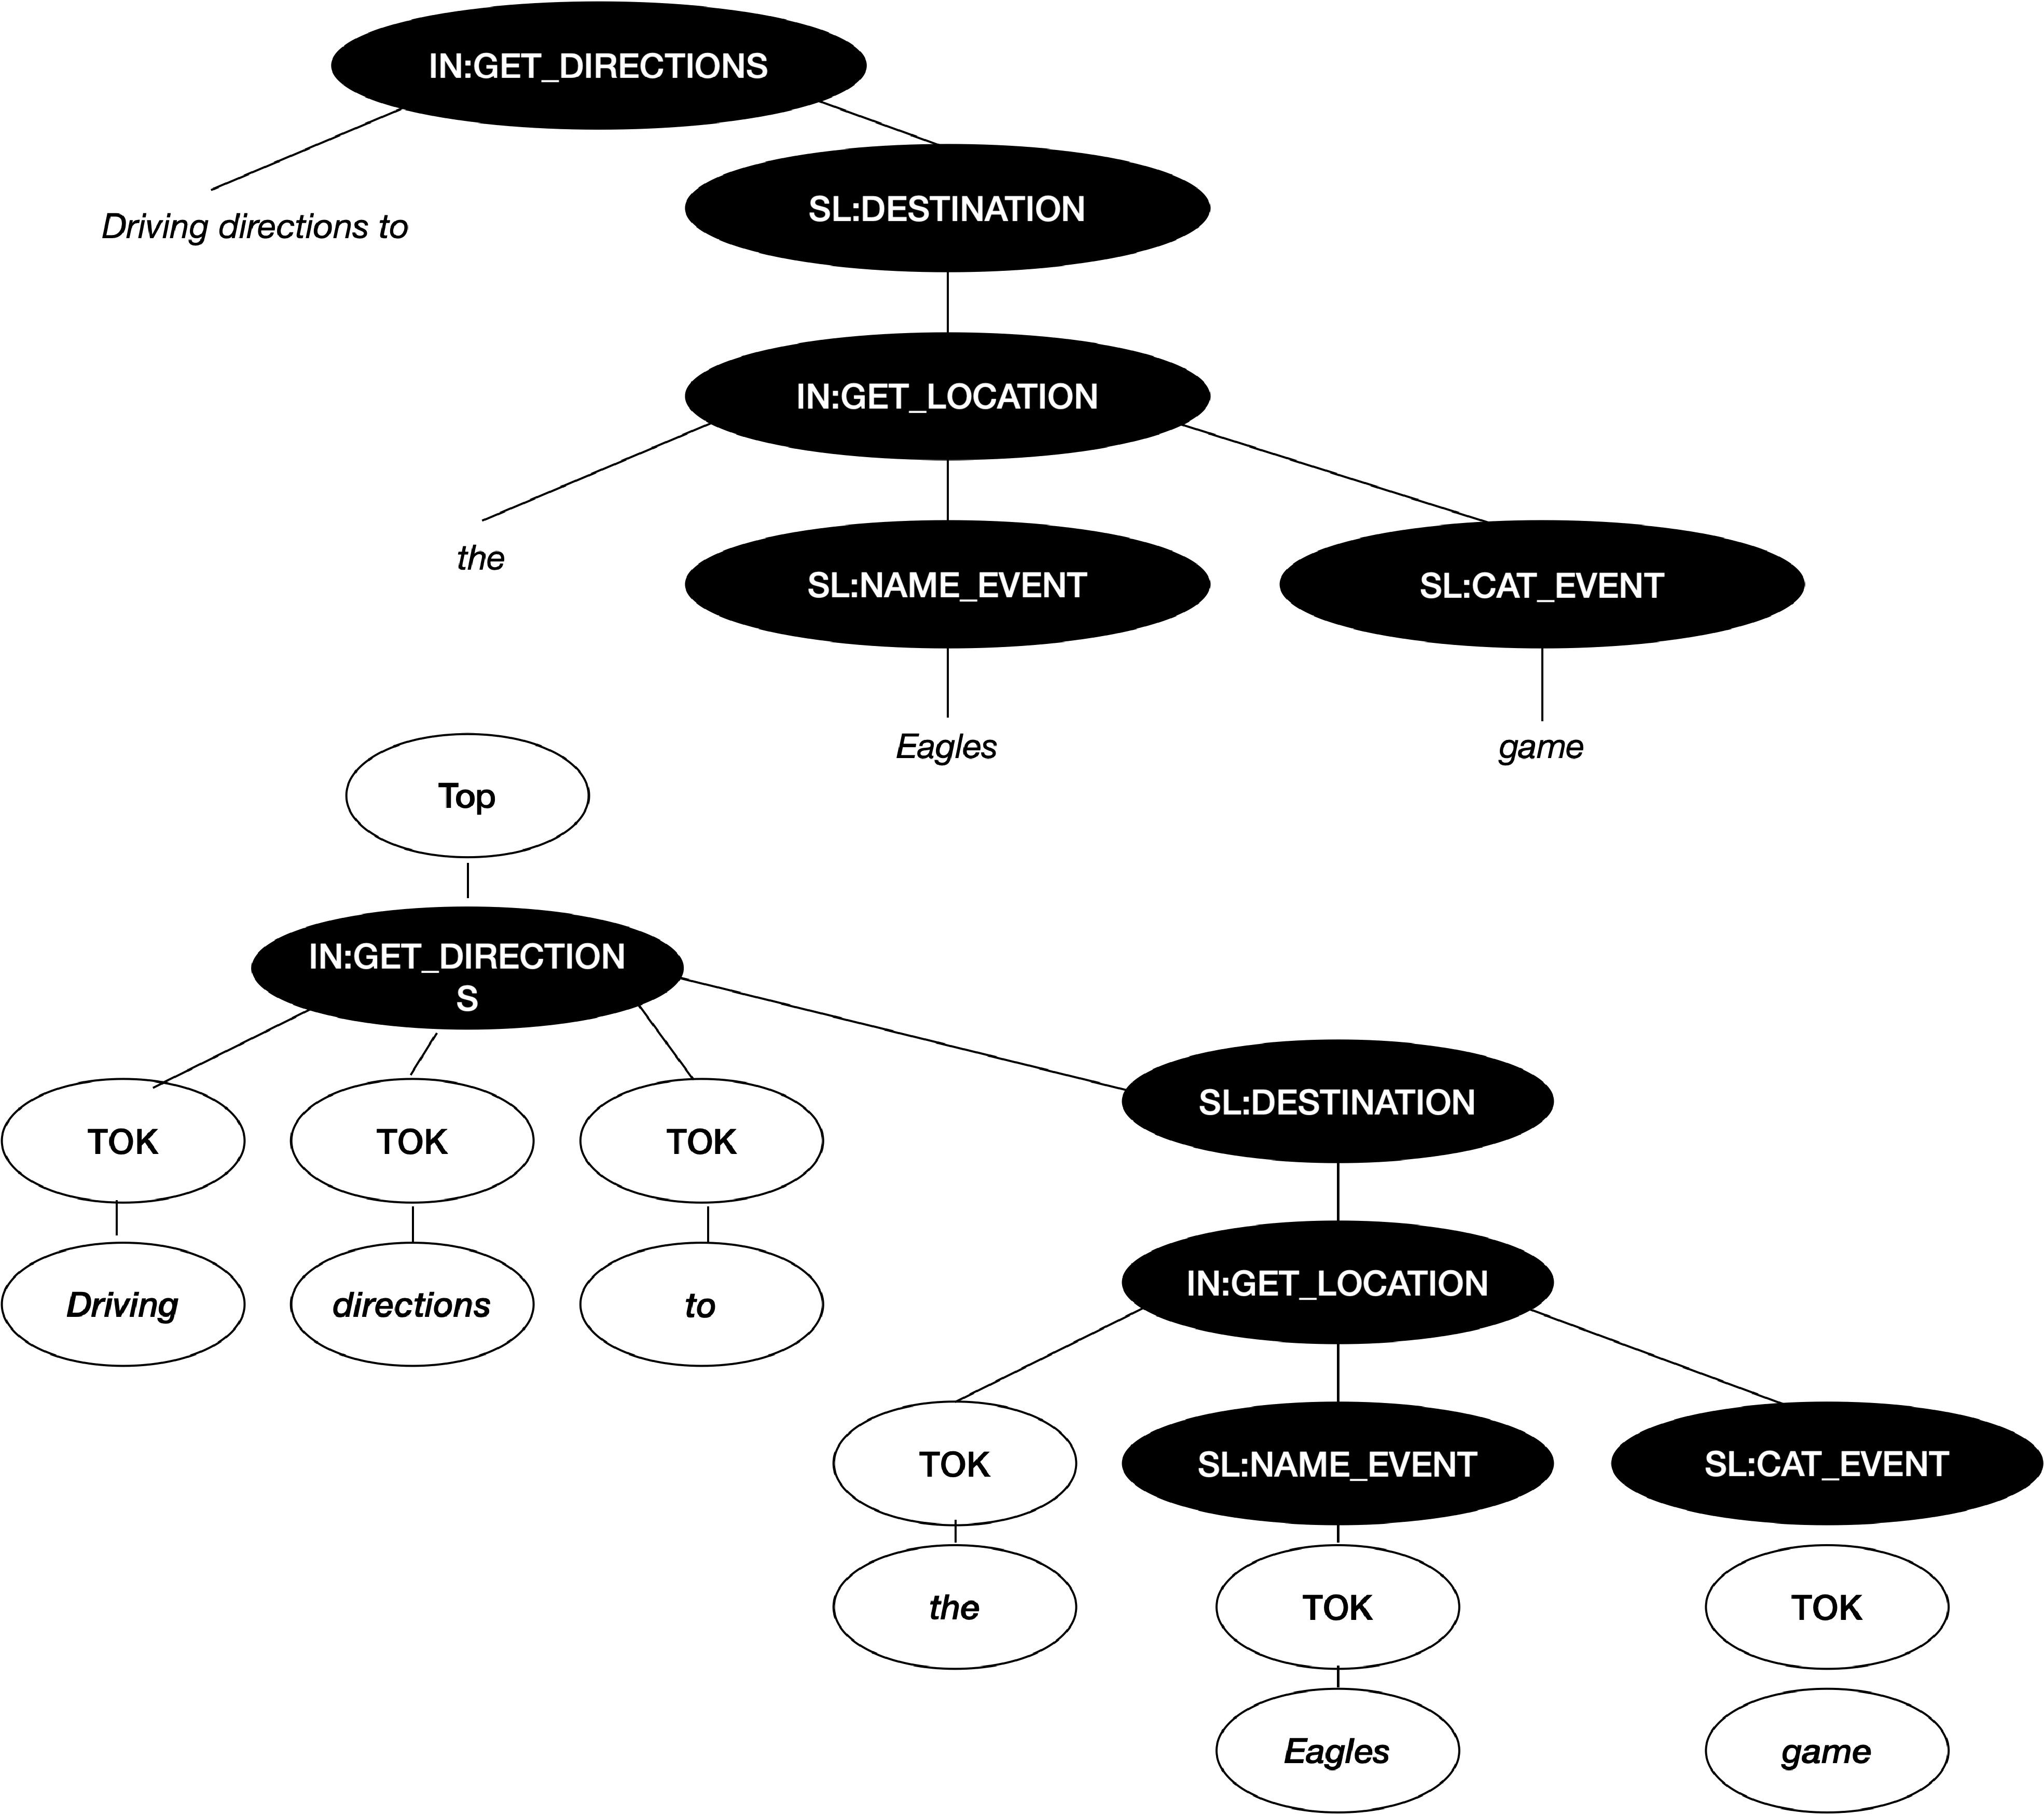
\includegraphics[width=0.90\textwidth]{TOP-to-CT.pdf}
\caption{\label{fig:TOP-to-CT} TOP to Constituent Tree Transformation
  for the utterance ``Driving directions to the Eagles game"}
\end{figure}

%%% Local Variables:
%%% mode: latex
%%% TeX-master: "../../thesis-main.ltx"
%%% End:
